\setchapterpreamble{\dictum[David Hilbert, \textit{Über das
  Unendliche}]{``No one shall expel us from the paradise that Cantor
has created.''}}
\chapter{Cardinality}
\begin{definition}[Cardinality]
  \addcontentsline{toc}{section}{Cardinality}
  \deflabel{cardinality-bijection}
  Let $S$ and $T$ be sets. Then, $\abs{S} = \abs{T}$ if and only if
  there is a bijection from $S$ to $T$.
\end{definition}

\begin{definition}[Cardinality cont.]
  \deflabel{cardinality-injection}
  $\abs{S} \leq \abs{T}$ if and only if there is an injection from $S$ to $T$.
\end{definition}

\begin{remark}
  Our definitions above introduce two fundamental relations on
  cardinality, i.e. $\size{S} = \size{T}$ and $\size{S} \leq
  \size{T}$. We need to make sure that these relations have the
  mathematical properties we expect them to have. That is, we want
  $\size{S} = \size{T}$ to be an equivalence relation and $\size{S}
  \leq \size{T}$ to be a partial order.

  For the relation $\size{S} = \size{T}$, it's easy to show that it
  defines an equivalence relation:
  \begin{itemize}
    \item Reflexivity: Every set has a bijection with itself, i.e.
      $\size{S} = \size{S}$.
    \item Symmetry: If there is a bijection $f$ from $S$ to $T$, then
      $f^{-1}$ is a bijection from $T$ to $S$, and thus $\size{T} = \size{S}$.
    \item Transitivity: If there are bijections $f$ from $S$ to $T$
      and $g$ from $T$ to $U$, then their composition $h = g \circ f$
      is a bijection from $S$ to $U$. Hence, $\size{S} = \size{U}$.
  \end{itemize}

  For the relation $\size{S} \leq \size{T}$, we must establish that
  it's a partial order:
  \begin{itemize}
    \item Reflexivity: Every set has an injection to itself, i.e.
      $\size{S} \leq \size{S}$.
    \item Transitivity: If there exist injections $f$ from $S$ to $T$
      and $g$ from $T$ to $U$, then their composition $h = g \circ f$
      is an injection from $S$ to $U$. Hence, $\size{S} \leq \size{U}$.
  \end{itemize}

  The remaining property, antisymmetry, is where things get
  interesting, since it's not immediately obvious. Antisymmetry means
  that if $\size{S} \leq \size{T}$ and $\size{T} \leq \size{S}$, then
  $\size{S} = \size{T}$. Using our definition, this translates to: If
  there is an injection from $S$ to $T$ and an injection from $T$ to
  $S$, then there should be a bijection between $S$ and $T$. This is
  exactly what the Schröder-Bernstein theorem
  (\thmref{schröder-bernstein}) guarantees.
\end{remark}

\begin{theorem}[Schröder-Bernstein theorem]
  \addcontentsline{toc}{section}{Schröder-Bernstein theorem}
  \thmlabel{schröder-bernstein}
  If there exist injections $f : A \to B$ and $g : B \to A$ between
  the sets $A$ and $B$, then there exists a bijection $h : A \to B$.

  In terms of the cardinality of the two sets, this implies that if
  $\size{A} \leq \size{B}$ and $\size{B} \leq \size{A}$, then
  $\size{A} = \size{B}$.
\end{theorem}

\begin{proof}
  The strategy is to partition $A$ and $B$ into components
  \[ A = X \cup X' \qquad \text{and} \qquad B = Y \cup Y' \]
  with $X \cap X' = \emptyset$ and $Y \cap Y' = \emptyset$, in such a
  way that $f$ is a surjection from $X$ to $Y$, and $g$ is a
  surjection from $Y'$ to $X'$. Achieving this would lead to a proof
  that there is a bijection $h$ from $A$ to $B$. Why? For all $x \in
  X'$, there exists a unique $y \in Y'$ satisfying $g(y) = x$. This
  means that there is a well-defined inverse function $g^{-1}(x) = y$
  that maps $X'$ to $Y'$. Setting
  \begin{align*}
    h(x) =
    \begin{cases}
      f(x) & \text{if $x \in X$} \\
      g^{-1}(x) & \text{if $x \in X'$}
    \end{cases}
  \end{align*}
  gives the desired bijection from $A$ to $B$.

  Now, let $X_1 = A \setminus g(B)$ and inductively define a sequence
  of sets by letting $X_{n + 1} = g(f(X_n))$.  Let $X = \bigcup_{n =
  1}^{\infty} X_n$ and $Y = \bigcup_{n = 1}^{\infty} f(X_n)$.

  To understand these definitions intuitively, observe that $X_1$
  consists of all elements in $A$ that are not in the image of $g$.
  Then $X_2$ consists of elements that are images under $g \circ f$
  of elements in $X_1$, and so on. Similarly, each $Y_n = f(X_n)$
  consists of the images of $X_n$ under $f$. The following diagram
  illustrates this construction and the relationship between these sets.

  \begin{tightfigure}
    \centering
    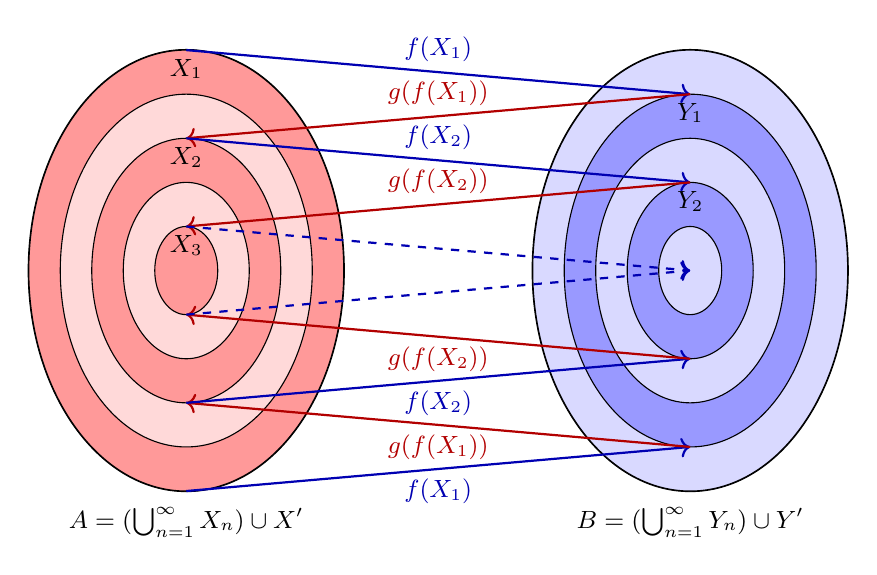
\begin{tikzpicture}[scale=0.8, every node/.style={font=\small}]

      % Draw outer ellipses for A and B
      \draw[thick] (0, 0) ellipse (2.5cm and 3.5cm);
      \draw[thick] (8, 0) ellipse (2.5cm and 3.5cm);

      % Recursive ellipses for A (shades of red)
      \foreach \i/\label/\shade in {0/X_1/red!40, 1//red!15,
      2/X_2/red!40, 3//red!15, 4/X_3/red!40} {
        \pgfmathsetmacro{\xradius}{2.5-\i*0.5}
        \pgfmathsetmacro{\yradius}{3.5-\i*0.7}
        \draw[fill=\shade] (0, 0) ellipse (\xradius cm and \yradius cm);
        \ifx\label\empty
        \else
        \node at (0, {\yradius-0.3}) {\(\label\)};
        \fi
      }

      % Recursive ellipses for B (shades of blue)
      \foreach \i/\label/\shade in {0//blue!15, 1/Y_1/blue!40,
      2//blue!15, 3/Y_2/blue!40, 4//blue!15} {
        \pgfmathsetmacro{\xradius}{2.5-\i*0.5}
        \pgfmathsetmacro{\yradius}{3.5-\i*0.7}
        \draw[fill=\shade] (8, 0) ellipse (\xradius cm and \yradius cm);
        \ifx\label\empty
        \else
        \node at (8, {\yradius-0.3}) {\(\label\)};
        \fi
      }

      % Arrows for f(X_1) = Y_1
      \draw[->, thick, blue!70!black] (0, 3.5) -- (8, 2.8)
      node[midway, above] {\(f(X_1)\)};
      \draw[->, thick, blue!70!black] (0, -3.5) -- (8, -2.8)
      node[midway, below] {\(f(X_1)\)};

      % Arrows for g(f(X_1)) = X_2.
      \draw[->, thick, red!70!black] (8, 2.8) -- (0, 2.1)
      node[midway, above] {\(g(f(X_1))\)};
      \draw[->, thick, red!70!black] (8, -2.8) -- (0, -2.1)
      node[midway, below] {\(g(f(X_1))\)};

      % Arrows for f(X_2) = Y_2.
      \draw[->, thick, blue!70!black] (0, 2.1) -- (8, 1.4)
      node[midway, above] {\(f(X_2)\)};
      \draw[->, thick, blue!70!black] (0, -2.1) -- (8, -1.4)
      node[midway, below] {\(f(X_2)\)};

      % Arrows for g(f(X_2)) = X_3.
      \draw[->, thick, red!70!black] (8, 1.4) -- (0, 0.7)
      node[midway, above] {\(g(f(X_2))\)};
      \draw[->, thick, red!70!black] (8, -1.4) -- (0, -0.7)
      node[midway, below] {\(g(f(X_2))\)};

      % Arrows for f(X_3) = Y_3.
      \draw[->, thick, dashed, blue!70!black] (0, 0.7) -- (8, 0)
      node[midway, above] {};
      \draw[->, thick, dashed, blue!70!black] (0, -0.7) -- (8, 0)
      node[midway, below] {};

      % Add labels for A and B
      \node at (0, -4) {\(A = (\bigcup_{n = 1}^{\infty} X_n) \cup X'\)};
      \node at (8, -4) {\(B = (\bigcup_{n = 1}^{\infty} Y_n) \cup Y'\)};
    \end{tikzpicture}
  \end{tightfigure}

  We show that $\set{X_n : n \in \NN}$ is a pairwise disjoint
  collection of subsets of $A$, while $\set{f(X_n) : n \in \NN}$ is a
  similar collection in $B$. To see that the sets $X_1, X_2, X_3,
  \dots$ are pairwise disjoint, note that $X_1 \cap X_n = \emptyset$
  for all $n \geq 2$ because $X_1 = A \setminus g(B)$ and $X_n
  \subseteq g(B)$. (Why? $f$ is a mapping from $A$ to $B$, so we have
    that $f(X_n) \subseteq B$, and thus $X_{n + 1} = g(f(X_n))
  \subseteq g(B)$.) In the general case of $X_n \cap X_m$ where $1 <
  n < m$, note that if $x \in X_n \cap X_m$ then $f^{-1}(g^{-1}(x))
  \in X_{n - 1} \cap X_{m - 1}$. Continuing in this way, we can show
  $X_1 \cap X_{m - n + 1}$ is not empty, which is a contradiction.
  Thus $X_n \cap X_m = \emptyset$. Just to be clear, the disjointness
  of the $X_n$ sets is not crucial to the overall proof, but it does
  help paint a clearer picture of how the sets $X$ and $X'$ are constructed.

  We show that $f$ is a surjection from $X$ to $Y$. This is
  straightforward. Each $x \in X$ comes from some $X_n$ and so $f(x)
  \in f(X_n) \subseteq Y$. Likewise, each $y \in Y$ is an element of
  some $f(X_n)$ and thus $y = f(x)$ for some $x \in X_n \subseteq X$.
  Thus $f : A \to B$ is a surjection.

  Let $y \in Y'$. Then $y \notin f(X_n)$ for all $n$ (by definition
  of $Y'$). We also conclude that $g(y) \notin X_{n + 1}$ for all
  $n$. (Why? Suppose if $g(y) \in X_{n + 1}$ for some $n$, then $g(y)
    \in g(f(X_n))$. That is, $g(y) = g(z)$ for some $z \in f(X_n)$, and
    since $g$ is injective, we have $y = z$ and thus $y \in f(X_n)$,
  which is a contradiction.) Clearly, $g(y) \notin X_1$ either
  (because $g(y) \subseteq g(B)$ and $X_1 = A \setminus g(B)$) and so
  $g$ is a mapping from $Y'$ to $X'$. To see that $g$ is a surjection
  from $Y'$ to $X'$, let $x \in X'$ be arbitrary. Because $X'
  \subseteq g(Y') \subseteq g(B)$, there exists $y \in B$ with $g(y)
  = x$. Could $y$ be an element of $Y$? No, because if $y \in Y$,
  $g(y)$ would be in $g(Y)$, and since $g(Y) \subseteq X$ (by
  definition of $Y$), this would mean $g(y) \in X$. But we're
  considering an $x \in X'$ with $g(y) = x$, so this is a
  contradiction as $X \cap X' = \emptyset$. Hence $y \in Y'$ and $g :
  Y' \to X'$ is a surjection.
\end{proof}

\begin{definition}[Cardinality cont.]
  \deflabel{cardinality-surjection}
  $\size{S} \geq \size{T}$ if and only if there is a surjection from $S$ to $T$.
\end{definition}

\begin{remark}
  Again, we must establish that $\size{S} \geq \size{T}$ defines a
  partial order. Reflexivity and transitivity are obvious. Now we
  will show antisymmetry. Suppose $\size{S} \geq \size{T}$ and
  $\size{T} \geq \size{S}$. Then, by definition, there are
  surjections from $S$ to $T$ and from $T$ to $S$. Using the axiom of
  choice, one can prove that there exists a surjection from $X$ to
  $Y$ if and only if there exists an injection from $Y$ to $X$. We
  conclude that $\size{T} \leq \size{S}$ and $\size{S} \leq
  \size{T}$, which implies $\size{S} = \size{T}$ by \thmref{schröder-bernstein}.
\end{remark}

\begin{theorem}[$\abs{\ZZ} = \abs{\NN}$]
  \addcontentsline{toc}{section}{$\abs{\ZZ} = \abs{\NN}$}
  \thmlabel{cardinality-of-z-equal-n}
  There are as many integers as there are natural numbers.
\end{theorem}

\begin{proof}
  Define the function $f : \NN \to \ZZ$ with
  \begin{align*}
    f(n) =
    \begin{cases}
      (n - 1) / 2 & \text{if $n$ is odd} \\
      - n / 2 & \text{if $n$ is even}.
    \end{cases}
  \end{align*}
  Clearly, $f$ is a bijection. (See the following diagram.)

  \begin{tightfigure}
    \centering
    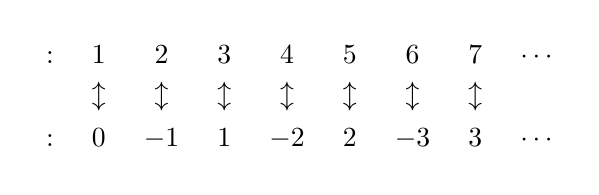
\begin{tikzpicture}[baseline]
      % Set up a matrix for the main content
      \matrix (m) [matrix of math nodes,
        column sep=0.25cm,
      row sep=0cm] {
        \NN : & 1 & 2 & 3 & 4 & 5 & 6 & 7 & \cdots \\
        & \updownarrow & \updownarrow & \updownarrow & \updownarrow &
        \updownarrow & \updownarrow & \updownarrow & \\
        \ZZ : & 0 & -1 & 1 & -2 & 2 & -3 & 3 & \cdots \\
      };
    \end{tikzpicture}
  \end{tightfigure}

  Hence, by \defref{cardinality-bijection}, $\size{\NN} = \size{\ZZ}$.
\end{proof}

\begin{remark}
  \thmref{cardinality-of-z-equal-n} also shows that two sets can have
  the same cardinality even if one is a proper subset of the other
  and the ``larger'' one even has infinitely many more elements than
  the ``smaller'' one. Make sure you take a moment to appreciate how
  remarkably, wonderfully weird this is.
\end{remark}

\begin{theorem}[$\abs{\QQ} = \abs{\NN}$]
  \addcontentsline{toc}{section}{$\abs{\QQ} = \abs{\NN}$}
  \thmlabel{cardinality-of-q-equal-n}
  There are as many rational numbers as there are natural numbers.
\end{theorem}

\begin{proof}
  Let $A_1 = \set{0}$ and for each $n \geq 2$, let $A_n$ be the set given by
  \[ A_n = \set{\pm\frac{p}{q} : \text{where $p, q \in \NN$ are in
  lowest terms with $p + q$ = n}}. \]
  The first few of these sets look like
  \[ A_1 = \set{0}, \qquad A_2 = \left\{\frac{1}{1},
    \frac{-1}{1}\right\}, \qquad A_3 = \left\{\frac{1}{2},
  \frac{-1}{2}, \frac{2}{1}, \frac{-2}{1}\right\}, \]
  \[ A_4 = \left\{\frac{1}{3}, \frac{-1}{3}, \frac{3}{1},
    \frac{-3}{1}\right\}, \qquad \text{and} \qquad A_5 =
    \left\{\frac{1}{4}, \frac{-1}{4}, \frac{2}{3}, \frac{-2}{3},
  \frac{3}{2}, \frac{-3}{2}, \frac{4}{1}, \frac{-4}{1}\right\}. \]
  The crucial observation is that each $A_n$ is finite and every
  rational number appears in exactly one of these sets. A bijection
  with $\NN$ is then achieved by consecutively listing the elements
  in each $A_n$.

  \begin{tightfigure}
    \centering
    \usetikzlibrary{decorations.pathreplacing}
    \begin{tikzpicture}[baseline]
      % Set up a matrix for the main content
      \matrix (m) [matrix of math nodes,
        column sep=0.25cm,
      row sep=0cm] {
        \NN : & 1 & 2 & 3 & 4 & 5 & 6 & 7 & 8 & 9 & 10 & 11 & 12 & \cdots \\
        & \updownarrow & \updownarrow & \updownarrow & \updownarrow &
        \updownarrow & \updownarrow & \updownarrow & \updownarrow &
        \updownarrow & \updownarrow & \updownarrow & \updownarrow & \\
        \QQ : &
        \makebox[\widthof{$-\dfrac{1}{1}$}][c]{$\vphantom{\dfrac{1}{1}}0$}
        & \dfrac{1}{1} &
        -\dfrac{1}{1} & \dfrac{1}{2} &
        -\dfrac{1}{2} & \dfrac{2}{1} & -\dfrac{2}{1} & \dfrac{1}{3} &
        -\dfrac{1}{3} & \dfrac{3}{1} & -\dfrac{3}{1} & \dfrac{1}{4} & \cdots \\
      };

      % Draw the underbraces
      \draw [decorate, decoration={brace, amplitude=6pt, mirror, raise=2pt}]
      (m-3-2.south west) -- (m-3-2.south east) node[midway, below=10pt] {$A_1$};

      \draw [decorate, decoration={brace, amplitude=6pt, mirror, raise=2pt}]
      (m-3-3.south west) -- (m-3-4.south east) node[midway, below=10pt] {$A_2$};

      \draw [decorate, decoration={brace, amplitude=6pt, mirror, raise=2pt}]
      (m-3-5.south west) -- (m-3-8.south east) node[midway, below=10pt] {$A_3$};

      \draw [decorate, decoration={brace, amplitude=6pt, mirror, raise=2pt}]
      (m-3-9.south west) -- (m-3-12.south east) node[midway,
      below=10pt] {$A_4$};
    \end{tikzpicture}
  \end{tightfigure}

  Admittedly, writing an explicit formula for this correspondence
  would be an awkward task, and attempting to do so is not the best
  use of time. What matters is that we see why every rational number
  appears in the correspondence exactly once. Given, say, $22/7$, we
  have that $22/7 \in A_{29}$. Because the set of elements in $A_1,
  \dots, A_{28}$ is finite, we can be confident that $22/7$
  eventually gets included in the sequence. The fact that this line
  of reasoning applies to any rational number $p/q$ is our proof that
  the correspondence is surjective. To verify that it is injective,
  we observe that the sets $A_n$ were constructed to be disjoint so
  that no rational number appears twice. This completes the proof.
\end{proof}

\begin{theorem}[$\abs{\RR} > \abs{\NN}$]
  \addcontentsline{toc}{section}{$\abs{\RR} > \abs{\NN}$}
  \thmlabel{cardinality-of-r-greater-than-n}
  There are more real numbers than natural numbers.
\end{theorem}

\begin{proof}
  Assume, for the sake of contradiction, that $\size{\RR} =
  \size{\NN}$, which implies that there is a bijection $f : \NN \to
  \RR$. What this suggests is that it is possible to enumerate the
  elements of $\RR$. If we let $x_1 = f(x_1)$, $x_2 = f(x_2)$, and so
  on, then the fact that $f$ is bijective (and thus surjective) means
  that we can write
  \[ \RR = \set{x_1, x_2, x_3, x_4, \dots} \tag{1} \]
  and be confident that every real number appears somewhere on the
  list. We will now use the nested intervals property
  (\thmref{nested-intervals-property}) to produce a real number that
  is not there.

  Let $I_1$ be a closed interval that does not contain $x_1$. Next,
  let $I_2$ be a closed interval, contained in $I_1$, which does not
  contain $x_2$. The existence of such $I_2$ is easy to verify.
  Certainly $I_1$ contains two smaller disjoint closed intervals, and
  $x_2$ can only be in one of these. In general, given an interval
  $I_n$, construct $I_{n + 1}$ to satisfy
  \begin{enumerate}
    \item $I_{n + 1} \subseteq I_n$ and
    \item $x_{n + 1} \notin I_{n + 1}$.
  \end{enumerate}
  We now consider the intersection $\bigcap_{n = 1}^{\infty} I_n$. If
  $x_k$ is some real number from the list in (1), then we have $x_k
  \notin I_k$, and it follows that
  \[ x_k \notin \bigcap_{n = 1}^{\infty} I_n. \]
  Now, we are assuming that the list in (1) contains every real
  number, and this leads to the conclusion that
  \[ \bigcap_{n = 1}^{\infty} I_n = \emptyset. \]
  However, the nested intervals property
  (\thmref{nested-intervals-property}) asserts that $\bigcap_{n =
  1}^{\infty} I_n \neq \emptyset$. So there is at least one $x \in
  \bigcap_{n = 1}^{\infty} I_n$ that, consequently, cannot be on the
  list in (1). This contradiction means that such an enumeration of
  $\RR$ is impossible, and we conclude that $\size{\RR} \neq \size{\NN}$.

  We are not done yet. We still have to show that $\size{\RR} \geq
  \size{\NN}$. This step is straightforward. Define the function $g :
  \RR \to \NN$ with
  \begin{align*}
    g(x) =
    \begin{cases}
      n & \text{if $x = n$ for some $n \in \NN$} \\
      0 & \text{otherwise}.
    \end{cases}
  \end{align*}
  This function maps each real number that is a natural number to
  itself, and all other real numbers to 0. Since every natural number
  is the image of at least one real number under $g$, the function is
  surjective. Therefore, by \defref{cardinality-surjection}, we have
  $\size{\RR} \geq \size{\NN}$. Combining this with our previous
  result that $\size{\RR} \neq \size{\NN}$, we conclude that
  $\size{\RR} > \size{\NN}$.
\end{proof}

\begin{definition}[Countable and uncountable sets]
  \addcontentsline{toc}{section}{Countable and uncountable sets}
  \deflabel{countable}
  A set $S$ is \vocab{countable} if
  \begin{enumerate}
    \item its cardinality $\size{S}$ is less than or equal to $\size{\NN}$.
    \item there exists an injection from $S$ to $\NN$.
    \item $S$ is empty or there exists a surjection $\NN$ to $S$.
    \item there exists a bijection from $S$ to a subset of $\NN$.
    \item $S$ is either finite or \textit{countably infinite}.
  \end{enumerate}
  All of the definitions above are equivalent.

  A set $S$ is \vocab{countably infinite} if its cardinality
  $\size{S}$ is exactly $\NN$.

  A set $S$ is \vocab{uncountable} if it is not countable. That is,
  its cardinality $\size{S}$ is greater than $\size{\NN}$.
\end{definition}

\begin{corollary}[$\NN$ is countable]
  \addcontentsline{toc}{section}{$\NN$ is countable}
  The set of natural numbers is countable.
\end{corollary}

\begin{corollary}[$\ZZ$ is countable]
  \addcontentsline{toc}{section}{$\ZZ$ is countable}
  The set of integers is countable.
\end{corollary}

\begin{corollary}[$\QQ$ is countable]
  \addcontentsline{toc}{section}{$\QQ$ is countable}
  \corlabel{q-is-countable}
  The set of rational numbers is countable.
\end{corollary}

\begin{corollary}[$\RR$ is uncountable]
  \addcontentsline{toc}{section}{$\RR$ is uncountable}
  \corlabel{r-is-uncountable}
  The set of real numbers is uncountable.
\end{corollary}

\begin{theorem}
  An uncountable collection of disjoint open intervals in $\RR$ cannot exist.
\end{theorem}

\begin{proof}
  We use contradiction. Suppose there exists an uncountable
  collection of disjoint open intervals in $\RR$. By the density of
  $\QQ$ in $\RR$ (\thmref{q-is-dense-in-r}), every open interval in
  $\RR$ contains at least one rational number. Therefore, there are
  uncountably many rational numbers. A contradiction of
  \corref{q-is-countable}. Hence, such a collection cannot exist.
\end{proof}

\begin{theorem}[Countable infinity is the smallest infinity]
  \addcontentsline{toc}{section}{Countable infinity is the smallest infinity}
  \thmlabel{countable-infinity-smallest}
  If $A \subseteq B$ and $B$ is countable, then $A$ is either
  countable or finite.
\end{theorem}

\begin{proof}
  $B$ is a countable set. Thus, there exists a bijection $f : \NN \to
  B$. Let $A \subseteq B$ be an infinite subset of $B$. We show that
  $A$ is countable. Let $n_1 \in \min\set{n \in \NN : f(n) \in A}$.
  As a start to a definition of $g : \NN \to A$, let $g(1) = f(n_1)$.
  Next let $n_2 = \min\set{n \in \NN : f(n) \in A \setminus
  \set{f(n_1)}}$ and let $g(2) = f(n_2)$. We inductively continue
  this process to produce a bijection $g$ from $\NN$ to $A$. In
  general, assume we have defined $g(k)$ for $k < m$, and let $g(m) =
  f(n_m)$ where $n_m = \min\set{n \in \NN : A \setminus \set{f(n_1),
  \dots, f(n_{k - 1})}}$.

  To show that $g$ is injective, observe that $m \neq m'$ implies
  $n_m \neq n_{m'}$ and it follows that $g(m) = f(n_m) \neq f(n_{m'})
  = g(m')$ because $f$ is injective. To show that $g$ is surjective,
  let $a \in A$ be arbitrary. Because $f$ is surjective, $a = f(n')$
  for some $n' \in \NN$. This means $n' \in \set{n : f(n) \in A}$ and
  as we inductively remove the minimal element, $n'$ must eventually
  be the minimum by at least the $(n' -1)$-th step.
\end{proof}

\begin{corollary}[$\size{\NN}$ is the smallest infinity]
  If $A \subseteq \NN$, then either $A$ is finite or $\size{A} = \size{\NN}$.
\end{corollary}

\begin{corollary}[Sizes of infinity]
  There are different sizes of infinity, with countable infinity
  being the smallest. Moreover, $\NN$, $\ZZ$ and $\QQ$ are countable
  while $\RR$ is uncountable.
\end{corollary}

\begin{theorem}[Countable union of countable sets is countable]
  \thmlabel{countable-union-countable}
  A countable union of countable sets is countable. More precisely:
  \begin{enumerate}
    \item If $A_1, A_2, \dots, A_m$ are each countable sets, then
      $A_1 \cup A_2 \cup \dots \cup A_m$ is countable.
    \item If $A_n$ is a countable set for each $n \in \NN$, then the
      set $\bigcup_{n = 1}^{\infty} A_n$ is also countable.
  \end{enumerate}
\end{theorem}

\begin{proof}
  First, we prove part 1 for two countable sets, $A_1$ and $A_2$.
  Some technicalities can be avoided by first replacing $A_2$ with
  the set $B_2 = A_2 \setminus A_1 = \set{x \in A_2 : x \notin A_1}$.
  The point of this is that the union $A_1 \cup B_2$ is equal to $A_1
  \cup A_2$ and the sets $A_1$ and $B_2$ are disjoint.

  Now, because $A_1$ is countable, there exists a bijection $f : \NN
  \to A_1$. If $B_2 = \emptyset$, then $A_1 \cup A_2 = A_1$ which we
  already know to be countable. If $B_2 = \set{b_1, b_2, \dots, b_m}$
  has $m$ elements then define $h : \NN \to A_1 \cup B_2$ via
  \begin{align*}
    h(n) =
    \begin{cases}
      b_n & \text{if $n \leq m$} \\
      f(n - m) & \text{if $n > m$}.
    \end{cases}
  \end{align*}
  The fact that $h$ is bijective follows immediately from the same
  property of $f$. If $B_2$ is infinite, then by
  \thmref{countable-infinity-smallest} it is countable, and so there
  exists a bijection $g : \NN \to B_2$. In this case we define $h :
  \NN \to A_1 \cup B_2$ by
  \begin{align*}
    h(n) =
    \begin{cases}
      f((n + 1) / 2) & \text{if $n$ is odd} \\
      g(n / 2) & \text{if $n$ is even}.
    \end{cases}
  \end{align*}
  Again, the proof that $h$ is bijective is derived directly from the
  fact that $f$ and $g$ are both bijections. Graphically, the
  correspondence takes the form

  \begin{tightfigure}
    \centering
    \begin{tikzpicture}[baseline]
      % Set up a matrix for the main content
      \matrix (m) [matrix of math nodes,
        column sep=0.25cm,
      row sep=0cm] {
        \makebox[\widthof{$A_1 \cup B_2 :$}][r]{$\NN :$} & 1 &
        2 & 3 & 4 & 5 & 6 & \cdots \\
        & \updownarrow & \updownarrow & \updownarrow & \updownarrow &
        \updownarrow & \updownarrow & \\
        A_1 \cup B_2 : & a_1 & b_1 & a_2 & b_2 & a_3 & b_3 & \cdots \\
      };
    \end{tikzpicture}
  \end{tightfigure}

  To prove the more general statement in part 1, we may use
  induction. We have just seen that the result holds for two
  countable sets. Now let's assume that the union of $m$ countable
  sets is countable, and show that the union of $m + 1$ countable
  sets is countable.

  Given $m + 1$ countable sets $A_1, A_2, \dots, A_{m + 1}$, we can write
  \[ A_1 \cup A_2 \cup \dots \cup A_{m + 1} = (A_1 \cup A_2 \cup
  \dots \cup A_m) \cup A_{m + 1}. \]
  Then $C_m = A_1 \cup \dots \cup A_m$ is countable by the induction
  hypothesis, and $C_m \cup A_{n + 1}$ is just the union of two
  countable sets which we know to be countable. This completes the
  proof for part 1.

  For part 2, induction cannot be used because we have an infinite
  number of sets. Instead, we show how arranging $\NN$ into the
  two-dimensional array
  \begin{align*}
    \begin{array}{cccccc}
      1  & 3  & 6  & 10 & 15 & \cdots \\
      2  & 5  & 9  & 14 & \cdots \\
      4  & 8  & 13 & \cdots \\
      7  & 12 & \cdots \\
      11 & \cdots \\
      \vdots \\
    \end{array}
  \end{align*}
  leads to a proof.

  Let's first consider the case where the sets $\set{A_n}$ are
  disjoint. In order to achieve bijection between $\NN$ and
  $\bigcup_{n = 1}^{\infty} A_n$, we first label the elements in each
  countable set $A_n$ as
  \[ A_n = \set{a_{n_1}, a_{n_2}, a_{n_3}, \dots}. \]
  Now arrange the elements of $\bigcup_{n = 1}^{\infty} A_n$ in an
  array similar to the one for $\NN$:
  \begin{align*}
    \begin{array}{cccccccc}
      A_1 & =  & a_{11} & a_{12} & a_{13} & a_{14} & a_{15} & \cdots \\
      A_2 & =  & a_{21} & a_{22} & a_{23} & a_{24} & \cdots &        \\
      A_3 & =  & a_{31} & a_{32} & a_{33} & \cdots &        &        \\
      A_4 & =  & a_{41} & a_{42} & \cdots &        &        &        \\
      A_5 & =  & a_{51} & \cdots &        &        &        &        \\
      & \vdots &        &        &        &        &        &        \\
    \end{array}
  \end{align*}
  This establishes a bijection $g : \NN \to \bigcup_{n = 1}^{\infty}
  A_n$ where $g(n)$ corresponds to the element $a_{jk}$ where $(j,
  k)$ is the row and column location of $n$ in the array for $\NN$.

  If the sets $\set{A_n}$ are not disjoint then our mapping may not
  be injective. In this case we could again replace $A_n$ with $B_n =
  A_n \setminus \set{A_1 \cup \dots \cup A_{n - 1}}$. Another
  approach is to use the previous argument to establish a bijection
  between $\bigcup_{n = 1}^{\infty} A_n$ and an infinite subset of
  $\NN$, and then appeal to \thmref{countable-infinity-smallest}.
  This completes the proof for part 2.
\end{proof}

\begin{theorem}[$\RR \setminus \QQ$ is uncountable]
  There are uncountably many irrational numbers.
\end{theorem}

\begin{proof}
  We use contradiction. Suppose $\RR \setminus \QQ$ is countable. By
  \thmref{countable-union-countable}, we know that a countable union
  of countable sets is countable, thus $(\RR \setminus \QQ) \cup \QQ
  = \RR$ is countable. A contradiction of \corref{r-is-uncountable}.
  Hence, $\RR \setminus \QQ$ is uncountable.
\end{proof}

\begin{theorem}[$\size{\QQ_+} = \size{\NN}$]
  \addcontentsline{toc}{section}{The winding bijection}
  There are as many positive rational numbers as there are natural numbers.
\end{theorem}

\begin{proof}
  The following diagram arranges the rational numbers (with some
  repetition) and illustrates our bijection, which we call the
  \textit{winding bijection}.

  \begin{tightfigure}
    \centering
    \usetikzlibrary{matrix, arrows.meta}
    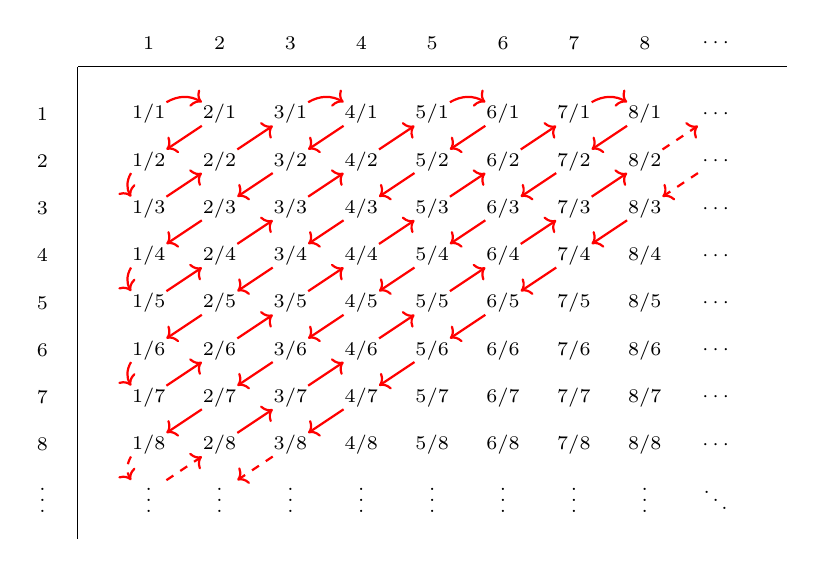
\begin{tikzpicture}[scale=0.6, font=\scriptsize]
      % Define the column and row headers
      \foreach \x in {1,...,8} {
        \node at (\x*1.5,0.5) {$\x$};
        \node at (-0.5*1.5,-\x) {$\x$};
      }
      \node at (9*1.5,0.5) {$\cdots$};
      \node at (-0.5*1.5,-9) {$\vdots$};

      % Draw horizontal line beneath the column headers
      \draw (0,0) -- (10*1.5,0);

      % Draw vertical line to the right of row headers
      \draw (0,0) -- (0,-10);

      % Create the matrix of fractions
      \foreach \x in {1,...,8} {
        \foreach \y in {1,...,8} {
          \node at (\x*1.5,-\y) {$\x/\y$};
        }
      }

      % Draw ellipsis
      \foreach \x in {1,...,8} {
        \node at (\x*1.5,-9) {$\vdots$};
      }
      \foreach \y in {1,...,8} {
        \node at (9*1.5,-\y) {$\cdots$};
      }
      \node at (9*1.5,-9) {$\ddots$};

      % To prevent arrows from touching the numbers
      \def\eps{0.25}

      % Draw the arrows
      \foreach \x in {1,...,7} {
        \foreach \y in {2,...,8} {
          \pgfmathparse{int(\x+\y)}
          \ifnum\pgfmathresult<12
          \pgfmathparse{int(mod(\pgfmathresult,2))}
          \ifnum\pgfmathresult=0
          % Diagonal arrows (upward)
          \draw[->,red,thick] (\x*1.5+\eps*1.5,-\y+\eps) --
          (\x*1.5+1*1.5-\eps*1.5,-\y+1-\eps);
          \else
          % Diagonal arrows (downward)
          \draw[->,red,thick] (\x*1.5+1*1.5-\eps*1.5,-\y+1-\eps) --
          (\x*1.5+\eps*1.5,-\y+\eps);
          \fi
          \fi
        }
      }

      % Draw curved arrows
      \foreach \x in {1,...,7} {
        \pgfmathparse{int(mod(\x,2))}
        \ifnum\pgfmathresult=1
        \draw[->,red,thick,bend left=30] (\x*1.5+\eps*1.5,-1+\eps) to
        (\x*1.5+1*1.5-\eps*1.5,-1+\eps);
        \fi
      }
      \foreach \y in {1,...,7} {
        \pgfmathparse{int(mod(\y,2))}
        \ifnum\pgfmathresult=0
        \draw[->,red,thick,bend right=30] (1*1.5-\eps*1.5,-\y-\eps) to
        (1*1.5-\eps*1.5,-\y-1+\eps);
        \fi
      }

      % Draw dashed arrows
      \draw[->,red,thick,dashed] (8*1.5+\eps*1.5,-2+\eps) to
      (9*1.5-\eps*1.5,-1-\eps);
      \draw[->,red,thick,dashed] (9*1.5-\eps*1.5,-2-\eps) to
      (8*1.5+\eps*1.5,-3+\eps);
      \draw[->,red,thick,dashed,bend right=30] (1*1.5-\eps*1.5,-8-\eps) to
      (1*1.5-\eps*1.5,-9+\eps);
      \draw[->,red,thick,dashed] (1*1.5+\eps*1.5,-9+\eps) to
      (2*1.5-\eps*1.5,-8-\eps);
      \draw[->,red,thick,dashed] (3*1.5-\eps*1.5,-8-\eps) to
      (2*1.5+\eps*1.5,-9+\eps);
    \end{tikzpicture}
  \end{tightfigure}

  Weaving through this chart, you are guaranteed to hit every
  positive rational number. So if you pair up 1 with the first number
  you hit, 2 with the second number you hit, 3 with the third, and so
  on, then every positive rational number is in a pair. Now, there's
  just one small problem: each rational number is actually hit more
  than once. The number $p/q$ will be written in positions $(p, q),
  (2p, 2q), (3p, 3q), \dots$. But the fix is easy: When you come
  across a number that has already been hit, just skip it. Clearly
  you won't run out of rational numbers, so this does indeed pair up
  everything. So
  \[ f(n) = \text{the $n$th new rational number you reach}. \]
  And that's it.
\end{proof}

\begin{theorem}[$\size{(0, 1)} > \size{\NN}$]
  \addcontentsline{toc}{section}{Cantor's diagonal argument}
  \thmlabel{cardinality-of-(0,1)-greater-than-n}
  There are more numbers in the open interval $(0, 1)$ than there are
  natural numbers.
\end{theorem}

We will demonstrate a clever argument known as \textit{Cantor's
diagonal argument}.

\begin{proof}
  We proceed by contradiction and assume that there does exist a
  function $f : \NN \to (0, 1)$ that is bijective. For each $m \in
  \NN$, $f(m)$ is a real number between 0 and 1, and we represent it
  using the decimal notation
  \[ f(m) = .a_{m1}a_{m2}a_{m3}a_{m4}a_{m5}\dots. \]
  What is meant here is that for each $m, n \in \NN$, $a_{mn}$ is the
  digit from the set $\set{0, 1, 2, \dots, 9}$ that represents the
  $n$th digit in the decimal expansion of $f(m)$. The bijection
  between $\NN$ and $(0, 1)$ can be summarized in the doubly indexed array
  \begin{align*}
    \begin{array}{ccccccccccc}
      \NN & & (0,1) & & & & & & & & \\
      \hline
      1 & \longleftrightarrow & f(1) & = & .\boldsymbol{a_{11}} &
      a_{12} & a_{13} & a_{14} & a_{15} & a_{16} & \cdots \\
      2 & \longleftrightarrow & f(2) & = & .a_{21} &
      \boldsymbol{a_{22}} & a_{23} & a_{24} & a_{25} & a_{26} & \cdots \\
      3 & \longleftrightarrow & f(3) & = & .a_{31} & a_{32} &
      \boldsymbol{a_{33}} & a_{34} & a_{35} & a_{36} & \cdots \\
      4 & \longleftrightarrow & f(4) & = & .a_{41} & a_{42} & a_{43}
      & \boldsymbol{a_{44}} & a_{45} & a_{46} & \cdots \\
      5 & \longleftrightarrow & f(5) & = & .a_{51} & a_{52} & a_{53}
      & a_{54} & \boldsymbol{a_{55}} & a_{56} & \cdots \\
      6 & \longleftrightarrow & f(6) & = & .a_{61} & a_{62} & a_{63}
      & a_{64} & a_{65} & \boldsymbol{a_{66}} & \cdots \\
      \vdots & \vdots & \vdots & \vdots & \vdots & \vdots & \vdots &
      \vdots & \vdots & \vdots & \ddots \\
    \end{array}
  \end{align*}
  The key assumption about this correspondence is that \textit{every}
  real number in $(0, 1)$ is assumed to appear somewhere on the list.
  Now for the pearl of the argument. Define a real number $x \in (0,
  1)$ with the decimal expansion $x = .b_1b_2b_3b_4\dots$ using the rule
  \begin{align*}
    b_n =
    \begin{cases}
      2 & \text{if $a_{nn} \neq 2$} \\
      3 & \text{if $a_{nn} = 2$}.
    \end{cases}
  \end{align*}
  Observe that $x = .b_1b_2b_3b_4\dots$ cannot be $f(1)$. $x$ also
  cannot be $f(2)$, and in general $x \neq f(n)$ for any $n \in \NN$.
  Therefore, the real number $x$ is nowhere on the list! This is a
  contradiction; clearly we were unable to pair up all the reals, if
  $x$ got left out.
\end{proof}

\begin{remark}
  Consider the following complaints about the proof of
  \thmref{cardinality-of-(0,1)-greater-than-n}.

  \begin{enumerate}
    \item Every rational number has a decimal expansion, so we could
      apply this same argument to show that the set of rational
      numbers between 0 and 1 is uncountable. However, because we
      know that any subset of $\QQ$ must be countable, the proof of
      \thmref{cardinality-of-(0,1)-greater-than-n} must be flawed.
    \item Some numbers have two different decimal representations
      (see \thmref{0.999...=1}). Specifically, any decimal expansion
      that terminates can also be written with repeating 9's. For
      instance, $1/2$ can be written as $.5$ or as $.4999\dots$.
      Doesn't this cause some problems?
  \end{enumerate}

  Are these complaints valid?
\end{remark}

Here's another proof of \thmref{cardinality-of-(0,1)-greater-than-n}
that I particular enjoy.

\begin{proofsketch}
  Imagine you were trying to map $\NN$ on to the real number line
  (which clearly has $\size{\RR}$ points).

  \begin{tightfigure}
    \centering
    \usetikzlibrary{arrows.meta}
    \begin{tikzpicture}[scale=1.5]
      % Define styles
      \tikzset{
        point/.style={circle, fill=black, inner sep=1.5pt}
      }

      % Bottom number line (real numbers)
      \draw[black, Latex-Latex] (0,0) -- (8,0);

      % Define positions for natural numbers and their corresponding images
      \def\posOne{1}
      \def\posTwo{2.5}
      \def\posThree{3.5}
      \def\posFour{4.5}
      \def\posFive{6}

      % Define the height of natural numbers (reduced from 2 to 1)
      \def\naturalHeight{1}

      % Draw natural numbers and points
      \foreach \x/\pos in {1/\posOne, 2/\posTwo, 3/\posThree,
      4/\posFour, 5/\posFive} {
        % Draw number label
        \node at (\pos,\naturalHeight+0.3) {$\x$};

        % Draw point
        \node[point] (p\x) at (\pos,\naturalHeight) {};
      }

      % Draw real number points
      \node[point] (r1) at (1,0) {};
      \node[point] (r2) at (3,0) {};
      \node[point] (r3) at (3.5,0) {};
      \node[point] (r4) at (5,0) {};
      \node[point] (r5) at (7,0) {};

      % Draw connecting lines - one arrow per natural number
      \draw[->] (p1) -- (r1);
      \draw[->] (p2) -- (r2);
      \draw[->] (p3) -- (r3);
      \draw[->] (p4) -- (r4);
      \draw[->] (p5) -- (r5);

      % Add ... for natural numbers
      \node at (7,\naturalHeight) {$\ldots$};
    \end{tikzpicture}
  \end{tightfigure}

  We aim to show that it is impossible for this map to be a
  bijection---there must be points on the real line that were missed.
  But instead of mapping just these points, let's make our job
  slightly harder. Around 1, let's put a little interval of length
  $\frac{1}{2}$. Around 2, let's put a little interval of length
  $\frac{1}{4}$. Around 3, let's place a little interval of length
  $\frac{1}{8}$. And so on. Now, when you map the points in $\NN$ to
  the real line, send over the intervals too (possibly some intervals
  will overlap; this is ok). We'll now prove that not only are there
  points on the real line that weren't mapped to, but there are even
  points that these intervals don't cover!

  \begin{tightfigure}
    \centering
    \usetikzlibrary{arrows.meta, positioning, fit, backgrounds, shadows}
    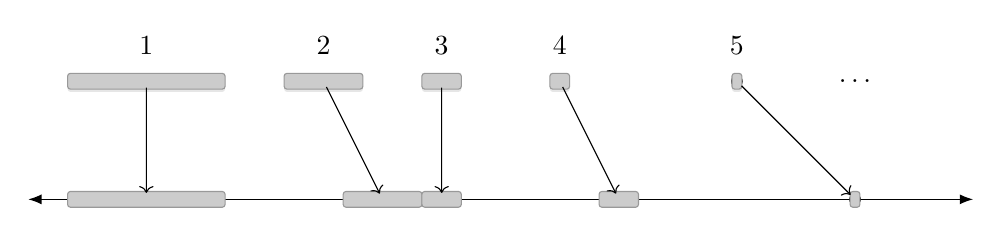
\begin{tikzpicture}[scale=1.5]
      % Define styles
      \tikzset{
        point/.style={circle, fill=black, inner sep=1.5pt},
        interval/.style={draw=black!40, fill=black!20, inner sep=1pt,
        minimum height=0.2cm, rectangle, rounded corners=1pt}
      }

      % Bottom number line (real numbers) - darker color
      \draw[black, Latex-Latex] (0,0) -- (8,0);

      % Define interval lengths
      \def\intervalOne{2}  % 1/2 unit
      \def\intervalTwo{1} % 1/4 unit
      \def\intervalThree{0.5} % 1/8 unit
      \def\intervalFour{0.25} % 1/16 unit
      \def\intervalFive{0.125} % 1/32 unit

      % Define the height of natural numbers (reduced from 2 to 1)
      \def\naturalHeight{1}

      % Draw natural numbers and their intervals with specified lengths
      % (no connecting line for natural numbers)
      \foreach \x/\pos/\intwidth in {1/1/\intervalOne,
        2/2.5/\intervalTwo, 3/3.5/\intervalThree, 4/4.5/\intervalFour,
      5/6/\intervalFive} {
        % Draw number label
        \node at (\pos,\naturalHeight+0.3) {$\x$};

        % Draw point
        \node[point] (p\x) at (\pos,\naturalHeight) {};

        % Draw interval around the point with specific width
        \node[interval, minimum width=\intwidth cm, drop
        shadow={shadow xshift=0pt, shadow yshift=-1pt, opacity=0.2}]
        (i\x) at (\pos,\naturalHeight) {};
      }

      % Draw real number points and their intervals with corresponding widths
      \node[point] (r1) at (1,0) {};
      \node[interval, minimum width=\intervalOne cm] at (1,0) {};

      \node[point] (r2) at (3,0) {};
      \node[interval, minimum width=\intervalTwo cm] at (3,0) {};

      \node[point] (r3) at (3.5,0) {};
      \node[interval, minimum width=\intervalThree cm] at (3.5,0) {};

      \node[point] (r4) at (5,0) {};
      \node[interval, minimum width=\intervalThree cm] at (5,0) {};

      \node[point] (r5) at (7,0) {};
      \node[interval, minimum width=\intervalFive cm] at (7,0) {};

      % Draw connecting lines - only one arrow per natural number
      \draw[->] (p1) -- (r1);
      \draw[->] (p2) -- (r2);
      \draw[->] (p3) -- (r3);
      \draw[->] (p4) -- (r4);
      \draw[->] (p5) -- (r5);

      % Add ... for natural numbers
      \node at (7,\naturalHeight) {$\ldots$};
    \end{tikzpicture}
  \end{tightfigure}

  See what happened? Our intervals' lengths add up to $\frac{1}{2} +
  \frac{1}{4} + \frac{1}{8} + \dots = 1$ (and with overlaps, their
    collective length when mapped to the real line may even be smaller
  than 1). But the whole real line has length $\infty$! So certainly
  there is no chance that all the points are covered; not only do the
  points of $\NN$ not cover the line, but even if we fatten them up
  with these intervals, those intervals don't even cover the real
  line! And any point that's in the ``$\infty - 1$'' portion of the
  real line that is not covered by an interval was certainly not
  mapped to. So we have all sorts of points that were missed, and so
  the mapping is far from being a bijection.

  And we could instead pick intervals that add up to 0.0001, or any
  other tiny number. This proof therefore provides a visualization of
  how we aren't just missing the one point that Cantor's
  diagonalization argument finds, but ``most'' points are missed.
\end{proofsketch}

\begin{theorem}[$\size{(0, 1)} = \size{\RR}$]
  \thmlabel{cardinality-of-(0,1)-equal-r}
  There are as many numbers in the open interval $(0, 1)$ as there
  are real numbers.
\end{theorem}

\begin{proofidea}
  The function $f(x) = (x-1/2)/(x-x^2)$ is a bijection from $(0, 1)$
  to $\RR$. This shows, by \defref{cardinality-bijection}, that
  $\size{(0, 1)} = \size{\RR}$.
\end{proofidea}

\begin{remark}
  \thmref{cardinality-of-(0,1)-equal-r} effectively establishes that
  \thmref{cardinality-of-r-greater-than-n} and
  \thmref{cardinality-of-(0,1)-greater-than-n} are equivalent.
\end{remark}

\begin{remark}
  We now know that $\size{\NN} < \size{\RR}$. Here's one natural
  question: Is there any infinity between these two? An astounding
  fact is that, based on the axioms of set theory (called ZFC),
  whether or not there exists such an infinity is
  \textit{unprovable}. And what I don't mean is that mathematicians
  are not smart enough to find the answer; no, I mean that they
  \textit{are} smart enough to have shown that \textit{no proof can
  possibly exist}. That's right, there are statements in math which
  are impossible to prove and also impossible to disprove (but we
  \textit{are} able to prove that they are unprovable, amazingly).

  This particular question is among the most famous in mathematical
  history. It was posed by Georg Cantor and is known as \textit{the
  continuum hypothesis}. It is the first of Hilbert's 23 problems—an
  influential list of unsolved problems that David Hilbert presented
  in 1900 at the International Congress of Mathematicians, setting
  the mathematical agenda for the 20th century. Decades later, Kurt
  Gödel's groundbreaking incompleteness theorems revealed that
  virtually every mathematical theory contains unprovable statements.

  ZFC set theory is the foundational framework upon which nearly all
  of modern mathematics is built. Gödel constructed a model of ZFC
  where the continuum hypothesis holds, while Paul Cohen later
  constructed a model where it fails. Together, their results
  established that the continuum hypothesis is independent of
  ZFC---it can be neither proved nor disproved within the system.
  Thus, the continuum hypothesis---which asks what is presumably a
  basic question about the infinite---is unprovable.
\end{remark}

\begin{hypothesis}[The continuum hypothesis]
  \addcontentsline{toc}{section}{The continuum hypothesis}
  There is no set whose cardinality is strictly between that of the
  naturals and the reals.
  \begin{align*}
    \size{\NN} < \size{S} < \size{\RR}.
  \end{align*}
\end{hypothesis}

\begin{theorem}[$\size{A} < \size{\power(A)}$]
  \addcontentsline{toc}{section}{$\size{A} < \size{\power(A)}$}
  \thmlabel{power-set-larger-cardinality}
  If $A$ is a set and $\power(A)$ is the power set of $A$, then
  \begin{align*}
    \size{A} < \size{\power(A)}.
  \end{align*}
\end{theorem}

\begin{proof}
  Assume for a contradiction that $\size{A} \geq \size{\power(A)}$.
  That is, assume that there is a surjection $f$ from $A$ to
  $\power(A)$. Since $f$ is a surjection, for every $T \subseteq A$,
  there is some element $t \in A$ where $f(t) = T$. To reach our
  contradiction, we will construct a set $B \subsetneq A$ which is not hit.

  For each $a$ there is one special property about the set $f(a)$
  that we are going to care about: Is $a \in f(a)$ or is $a \notin
  f(a)$? In general, consider the set of all elements $a$ such that
  $a \notin f(a)$, and call this set $B$:
  \[ B = \set{a \in A : a \notin f(a)}. \]
  By the above, if we can show that that there is no $b$ where $f(b)
  = B$, then we are done; we will have discovered an element of
  $\power(A)$ that was not hit by $f$, a contradiction.

  \underline{Claim.} There is no $b \in A$ such that $f(b) = B$.

  \underline{Proof of claim.} Assume for a contradiction that there
  does exist some $b \in A$ such that $f(b) = B$. Note by the
  definition of $B$ that
  \[ \text{$b \in B$ if and only if $b \notin f(b)$}. \]
  But since we assumed that $f(b) = B$, this is equivalent to
  \[ \text{$b \in f(b)$ if and only if $b \notin f(b)$}, \]
  which is clearly a contradiction.
\end{proof}

\begin{corollary}[There exist infinitely many infinities]
  \addcontentsline{toc}{section}{There exist infinitely many infinities}
  There exist infinitely many distinct infinite cardinalities.
\end{corollary}

\begin{proof}
  By \thmref{power-set-larger-cardinality}, the following is a chain
  of distinct infinite cardinalities
  \[ \size{\NN} < \size{\power(\NN)} < \size{\power(\power(\NN))} <
    \size{\power(\power(\power(\NN)))} <
  \size{\power(\power(\power(\power(\NN))))} < \dots.\]
\end{proof}
